\documentclass[tikz,border=5mm]{standalone}

\usepackage[T1]{fontenc}
\usepackage[sfdefault,sb]{plex-sans}
\usepackage{xcolor}
\usepackage{tikz}

\usetikzlibrary{arrows.meta,positioning}

\renewcommand*\familydefault{\sfdefault}

\definecolor{foundationfill}{HTML}{2E64FE}
\definecolor{foundationstroke}{HTML}{153E7E}
\definecolor{corefill}{HTML}{0033CC}
\definecolor{corestroke}{HTML}{001F7A}
\definecolor{advancedfill}{HTML}{000066}
\definecolor{advancedstroke}{HTML}{000033}
\definecolor{edgegray}{HTML}{475569}
\definecolor{crosslinkgray}{HTML}{64748B}

\begin{document}
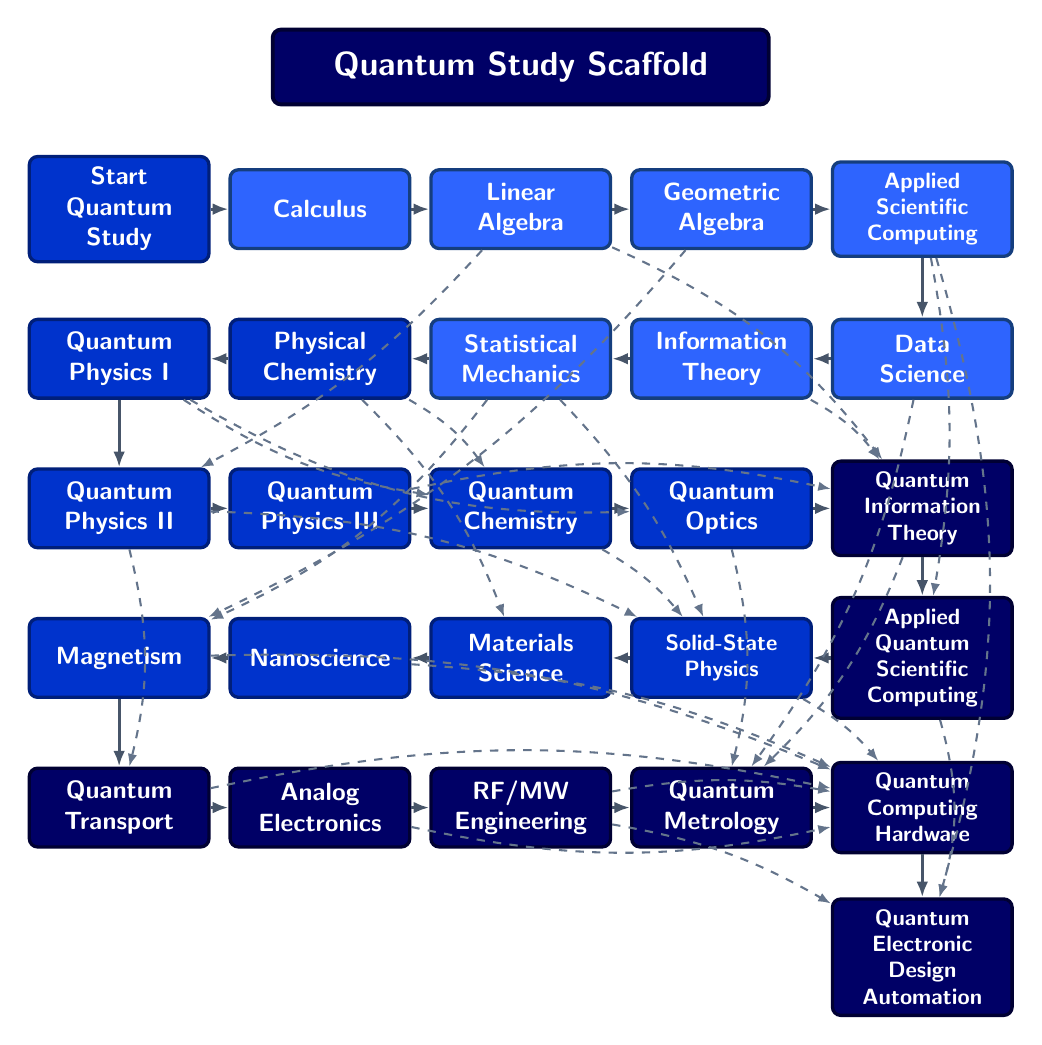
\begin{tikzpicture}[
  x=2.55cm,
  y=-1.90cm,
  every node/.style={
    rectangle,
    rounded corners=3pt,
    align=center,
    inner sep=4pt,
    minimum width=2.15cm,
    minimum height=1.00cm,
    text width=2.00cm,
    font=\small
  },
  scaffold/.style={
    -{Latex[length=2mm]},
    draw=edgegray,
    line width=1.15pt
  },
  crosslink/.style={
    -{Latex[length=1.6mm]},
    draw=crosslinkgray,
    line width=0.75pt,
    dashed
  },
  foundation/.style={
    draw=foundationstroke,
    fill=foundationfill,
    text=white,
    line width=1.2pt,
    font=\bfseries\small
  },
  longfoundation/.style={
    draw=foundationstroke,
    fill=foundationfill,
    text=white,
    line width=1.2pt,
    font=\bfseries\footnotesize
  },
  core/.style={
    draw=corestroke,
    fill=corefill,
    text=white,
    line width=1.2pt,
    font=\bfseries\small
  },
  longcore/.style={
    draw=corestroke,
    fill=corefill,
    text=white,
    line width=1.2pt,
    font=\bfseries\footnotesize
  },
  advanced/.style={
    draw=advancedstroke,
    fill=advancedfill,
    text=white,
    line width=1.2pt,
    font=\bfseries\small
  },
  longadvanced/.style={
    draw=advancedstroke,
    fill=advancedfill,
    text=white,
    line width=1.2pt,
    font=\bfseries\footnotesize
  },
  title/.style={
    draw=advancedstroke,
    fill=advancedfill,
    text=white,
    line width=1.4pt,
    font=\bfseries\large,
    minimum width=6.3cm,
    minimum height=0.95cm,
    text width=5.9cm
  }
]

\node[title] (title) at (2,-0.95) {Quantum Study Scaffold};

% Row 1, left to right
\node[core]           (start)   at (0,0) {Start\\Quantum Study};
\node[foundation]     (calc)    at (1,0) {Calculus};
\node[foundation]     (linalg)  at (2,0) {Linear\\Algebra};
\node[foundation]     (geoalg)  at (3,0) {Geometric\\Algebra};
\node[longfoundation] (scicomp) at (4,0) {Applied\\Scientific\\Computing};

% Row 2, right to left
\node[foundation] (datasci)  at (4,1) {Data\\Science};
\node[foundation] (info)     at (3,1) {Information\\Theory};
\node[foundation] (statmech) at (2,1) {Statistical\\Mechanics};
\node[core]       (physchem) at (1,1) {Physical\\Chemistry};
\node[core]       (qm1)      at (0,1) {Quantum\\Physics I};

% Row 3, left to right
\node[core]         (qm2)     at (0,2) {Quantum\\Physics II};
\node[core]         (qm3)     at (1,2) {Quantum\\Physics III};
\node[core]         (qchem)   at (2,2) {Quantum\\Chemistry};
\node[core]         (qoptics) at (3,2) {Quantum\\Optics};
\node[longadvanced] (qinfo)   at (4,2) {Quantum\\Information\\Theory};

% Row 4, right to left
\node[longadvanced] (aqsc)      at (4,3) {Applied Quantum\\Scientific\\Computing};
\node[longcore]     (solid)     at (3,3) {Solid-State\\Physics};
\node[core]         (materials) at (2,3) {Materials\\Science};
\node[core]         (nano)      at (1,3) {Nanoscience};
\node[core]         (mag)       at (0,3) {Magnetism};

% Row 5, left to right
\node[advanced]     (qtransport) at (0,4) {Quantum\\Transport};
\node[advanced]     (analog)     at (1,4) {Analog\\Electronics};
\node[advanced]     (rfmw)       at (2,4) {RF/MW\\Engineering};
\node[advanced]     (qmet)       at (3,4) {Quantum\\Metrology};
\node[longadvanced] (qhw)        at (4,4) {Quantum\\Computing\\Hardware};

% Row 6, final implementation layer
\node[longadvanced] (qeda) at (4,5) {Quantum\\Electronic\\Design\\Automation};

% Main serpentine scaffold path
\draw[scaffold] (start) -- (calc);
\draw[scaffold] (calc) -- (linalg);
\draw[scaffold] (linalg) -- (geoalg);
\draw[scaffold] (geoalg) -- (scicomp);

\draw[scaffold] (scicomp) -- (datasci);
\draw[scaffold] (datasci) -- (info);
\draw[scaffold] (info) -- (statmech);
\draw[scaffold] (statmech) -- (physchem);
\draw[scaffold] (physchem) -- (qm1);

\draw[scaffold] (qm1) -- (qm2);
\draw[scaffold] (qm2) -- (qm3);
\draw[scaffold] (qm3) -- (qchem);
\draw[scaffold] (qchem) -- (qoptics);
\draw[scaffold] (qoptics) -- (qinfo);

\draw[scaffold] (qinfo) -- (aqsc);
\draw[scaffold] (aqsc) -- (solid);
\draw[scaffold] (solid) -- (materials);
\draw[scaffold] (materials) -- (nano);
\draw[scaffold] (nano) -- (mag);

\draw[scaffold] (mag) -- (qtransport);
\draw[scaffold] (qtransport) -- (analog);
\draw[scaffold] (analog) -- (rfmw);
\draw[scaffold] (rfmw) -- (qmet);
\draw[scaffold] (qmet) -- (qhw);

\draw[scaffold] (qhw) -- (qeda);

% Conceptual cross-links
\draw[crosslink] (linalg) to[bend left=10] (qm2);
\draw[crosslink] (linalg) to[bend left=14] (qinfo);
\draw[crosslink] (geoalg) to[bend left=12] (mag);

\draw[crosslink] (scicomp) to[bend left=10] (aqsc);
\draw[crosslink] (scicomp) to[bend left=16] (qeda);
\draw[crosslink] (datasci) to[bend left=12] (qmet);
\draw[crosslink] (info) to[bend left=12] (qinfo);

\draw[crosslink] (statmech) to[bend left=10] (solid);
\draw[crosslink] (statmech) to[bend left=14] (mag);
\draw[crosslink] (physchem) to[bend left=12] (qchem);
\draw[crosslink] (physchem) to[bend left=12] (materials);

\draw[crosslink] (qm1) to[bend right=12] (qchem);
\draw[crosslink] (qm1) to[bend right=16] (qoptics);
\draw[crosslink] (qm2) to[bend left=12] (solid);
\draw[crosslink] (qm2) to[bend left=14] (qtransport);
\draw[crosslink] (qm3) to[bend left=12] (qinfo);

\draw[crosslink] (qchem) to[bend left=10] (solid);
\draw[crosslink] (qoptics) to[bend left=14] (qmet);
\draw[crosslink] (qinfo) to[bend left=12] (qmet);

\draw[crosslink] (solid) to[bend left=10] (qhw);
\draw[crosslink] (nano) to[bend left=10] (qhw);
\draw[crosslink] (qtransport) to[bend left=12] (qhw);
\draw[crosslink] (mag) to[bend left=12] (qhw);

\draw[crosslink] (analog) to[bend right=12] (qhw);
\draw[crosslink] (rfmw) to[bend left=10] (qhw);
\draw[crosslink] (rfmw) to[bend left=10] (qeda);
\draw[crosslink] (aqsc) to[bend left=16] (qeda);

\end{tikzpicture}
\end{document}
